\documentclass[a4paper, 12pt]{article}
\usepackage[utf8x]{inputenc}
\usepackage{cmap}
\usepackage[english, russian]{babel}
\usepackage{indentfirst}
\usepackage[left=20mm, top=20mm, right=20mm, bottom=20mm]{geometry}
\usepackage{tikz}
\usepackage{float}
\usepackage{amsmath, amsfonts, amssymb}
\usepackage{graphicx}
\usepackage{fancybox, fancyhdr}
\usepackage{hyperref}
\usepackage{listings}
\usepackage{caption}
\usepackage{subcaption}
\usepackage{xcolor}
\pagestyle{fancy}
\fancyhf{}
\fancyhead[L]{Лабораторная работа №1}
\fancyhead[R]{Математическая статистика}
\fancyfoot[C]{\thepage}
\graphicspath{{images/}}
\usetikzlibrary{patterns}
\definecolor{LightGray}{gray}{0.95}
\definecolor{LightGray2}{gray}{0.7}
\lstdefinestyle{code}{
    language=Python, % replace with needed language
    basicstyle=\footnotesize\ttfamily,
    backgroundcolor=\color{LightGray},
    showspaces=false,
    showstringspaces=false,
    showtabs=false,
    tabsize=4,
    captionpos=b,
    breaklines=true,
    breakatwhitespace=false,
    frame=single,
    rulecolor=\color{LightGray2},
    linewidth=\linewidth,
    keywordstyle=\color{blue}\bfseries,
    commentstyle=\color{green!40!black},
    stringstyle=\color{purple},
    escapeinside={\%*}{*)},
    inputencoding=utf8x,
    xleftmargin=0pt,
    framexleftmargin=0pt,
    framexrightmargin=0pt
}
\lstset{style=code}
\hypersetup{
    colorlinks=true,
    linkcolor=blue,
    filecolor=magenta,
    urlcolor=cyan,
    pdftitle={contents setup},
    pdfpagemode=FullScreen,
}
\setlength{\parskip}{1.5mm}
\setlength{\headheight}{15pt}
\setlength{\footskip}{15pt}
\allowdisplaybreaks
\DeclareMathOperator{\sinc}{sinc}
\newcommand{\frc}[2]{\raisebox{2pt}{$#1$}\big/\raisebox{-3pt}{$#2$}}

\begin{document}
    \begin{titlepage}

        \begin{center}
        
\includegraphics[width=0.3\textwidth]{itmo.png} % requires itmo.png in /images folder
        \vfill
        
        Федеральное государственное автономное образовательное учреждение высшего образования
        «Национальный Исследовательский Университет ИТМО»\\
        
        \vfill
        {\large\bf ЛАБОРАТОРНАЯ РАБОТА №1}\\
        {\large\bf ПРЕДМЕТ «МАТЕМАТИЧЕСКАЯ СТАТИСТИКА»}\\
        {\large\bf ТЕМА «ХАРАКТЕРИСТИКИ РАСПРЕДЕЛЕНИЯ И ОЦЕНКА ПАРАМЕТРА»}\\
        Вариант 4, 2
        \vfill

        \begin{flushright}
            \begin{minipage}{.45\textwidth}
            {
                \hbox{Преподаватель: Лимар И. А.}
                \hbox{Студент: Румянцев А. А.}
                \hbox{Поток: Мат Стат 31.2}
                \hbox{}
                \hbox{Факультет: СУиР}
                \hbox{Группа: R3341}
            }
            \end{minipage}
        \end{flushright}
        
        \vfill
                
        Санкт-Петербург\\
        2024
        \end{center}
    \end{titlepage}
    
    \tableofcontents

    \newpage
    \section{Задание 1}
    \subsection{Условие}
    В файле mobile\_{phones}.csv приведены данные о мобильных телефонах. В сколько моделей
    можно вставить 2 сим-карты, сколько поддерживают 3-G, каково наибольшее число ядер
    у процессора? Рассчитайте выборочное среднее, выборочную дисперсию, выборочную медиану
    и выборочную квантиль порядка 2/5, построить график эмпирической функции
    распределения, гистограмму и box-plot для емкости аккумулятора для всей совокупности
    и в отдельности для поддерживающих/не поддерживающих Wi-Fi


    \subsection{Выполнение}
    Для начала импортируем необходимые библиотеки
    \begin{lstlisting}[label=import, caption={Импортирование библиотек}]
    import numpy as np
    import pandas as pd
    import matplotlib.pyplot as plt
    \end{lstlisting}


    Теперь считаем таблицу по ссылке на представленный гугл-диск в переменную df
    \begin{lstlisting}[label=read, caption={Считывание таблицы}]
    url='https://drive.google.com/file/d/1O4rFr9xg9aFmkjx4-hl_XOc5O9q65_EW\
        /view?usp=sharing'
    url='https://drive.google.com/uc?id=' + url.split('/')[-2]
    df = pd.read_csv(url)
    \end{lstlisting}


    В колонках <<dual\_{sim}>> и <<three\_{g}>> наличие или отсутствие параметра определяется
    единицей или нулем соответственно, следовательно, просуммировав значения в этих столбцах,
    получим количество моделей с наличием данных параметров. Для ядер просто выведем максимум
    из столбца. Используем методы библиотеки \texttt{pandas} -- \texttt{sum} и \texttt{max}
    \begin{lstlisting}[label=3q, caption={Код на ответы на первые три вопроса}]
    # how many models can you insert 2 SIM cards into?
    dual_sim_count = df['dual_sim'].sum()
    print(f'dual_sim_count={dual_sim_count}')
        
    # how many models support 3-G?
    three_g_count = df['three_g'].sum()
    print(f'three_g_count={three_g_count}')
        
    # what is the highest number of cores a processor has?
    max_cores = df['n_cores'].max()
    print(f'max_cores={max_cores}')
    \end{lstlisting}

    
    Получим следующий вывод в консоль
    \begin{lstlisting}[label=3qa, caption={Вывод в консоль: ответы на первые три вопроса}]
    dual_sim_count=1019
    three_g_count=1523
    max_cores=8
    \end{lstlisting}


    Для расчета необходимых характеристик я написал отдельный метод, куда достаточно
    передать выборку и ее именование для удобного вывода в консоль. Используем методы
    библиотеки \texttt{pandas} -- \texttt{mean} посчитает выборочное среднее,
    \texttt{var} выборочную дисперсию, \texttt{median} выборочную медиану и \texttt{quantile}
    с параметром \texttt{q=2/5} квантиль порядка 2/5
    \begin{lstlisting}[label=mvals, caption={Код для подсчета основных характеристик}]
    # calculating the main values
    def calculate_print_values(df: pd.Series, name: str):
        mean = df.mean()
        print(f'mean_{name}={mean}')
        
        var = df.var()
        print(f'var_{name}={var}')
        
        median = df.median()
        print(f'median_{name}={median}')
        
        quantile_2d5 = df.quantile(q=2/5)
        print(f'quantile_2/5_{name}={quantile_2d5}')
    \end{lstlisting}


    Зададим сразу три выборки -- всю, только модели с наличием Wi-Fi и только с отсутствием.
    Для составления выборок с конкретным значением требуемого параметра берем нужный столбец
    и составляем построчную связку индекс-булеан, где значением будет являться результат проверки заданного условия.
    Обращаемся к исходной таблице по этой связке и получаем новую таблицу только с теми строками, для которых по индексу
    значение было равным \texttt{True}, то есть условие выполнилось. Далее от полученной таблицы отбираем столбец по условию задания.
    Для удобного вывода добавим метод разделитель, который будем вызывать между операциями с выборками.
    Вызовем подсчитывающий метод три раза для трех выборок
    \begin{lstlisting}[label=mvals2, caption={Подготовка для удобного и быстрого получения результатов}]
    # common separator between unrelated outputs
    def print_separate():
        print('----------------')

    # the entire sample
    all_battery = df['battery_power']
    calculate_print_values(all_battery, name='all_battery')

    print_separate()

    # selection with the condition of wifi availability
    wifi_table = df[df['wifi']==1]
    wifi_battery = wifi_table['battery_power']
    calculate_print_values(wifi_battery, name='wifi_battery')

    print_separate()

    # selection with the condition of wifi unavailability
    nowifi_table = df[df['wifi']==0]
    no_wifi_battery = nowifi_table['battery_power']
    calculate_print_values(no_wifi_battery, name='no_wifi_battery')
    \end{lstlisting}


    С заданными ранее параметрами получаем следующий вывод в консоль
    \begin{lstlisting}[label=mvalsout, caption={Вывод в консоль: посчитанные основные характеристики}]
    mean_all_battery=1238.5185
    var_all_battery=193088.35983766883  
    median_all_battery=1226.0
    quantile_2/5_all_battery=1076.0     
    ----------------
    mean_wifi_battery=1234.9043392504932
    var_wifi_battery=190296.40051422242 
    median_wifi_battery=1233.0
    quantile_2/5_wifi_battery=1077.8000000000002
    ----------------
    mean_no_wifi_battery=1242.235294117647      
    var_no_wifi_battery=196128.43798148702      
    median_no_wifi_battery=1222.0
    quantile_2/5_no_wifi_battery=1076.0
    \end{lstlisting}


    Теперь построим графики в соответствии с заданием.
    Напишем метод, который принимает выборку и название графика -- таким образом, достаточно
    будет вызвать метод для каждой выборки и получить все графики. Используем библиотеку 
    \texttt{matplotlib} для отрисовки, \texttt{pandas} для подсчета необходимых данных.
    Для построения графика эмпирической функции распределения находим
    по сортированным данным без сохранения индексов связку ключ-значение, где ключ --
    \texttt{battery\_{power}}, значение -- вероятность встретить именно такую \texttt{battery\_{power}}.
    После составляем кумулятивные суммы по этим вероятностям. Для гистограммы определяем
    количество интервалов правилом Стёрджеса: $n=1+\log_2{N}$ и округляем вниз
    \begin{lstlisting}[label=graphs, caption={Код для построения необходимых графиков}]
    # plotting basic graphs
    def show_graphs(df: pd.Series, name='sample'):
        # the resulting axis will be labeled 0, 1, ..., n - 1
        sorted_ = df.sort_values(ignore_index=True)

        # normalize for proportions (probabilities) instead of freqs
        # sorting by DataFrame column values (not by freqs)
        idx_prob = sorted_.value_counts(normalize=True, sort=False)

        # parsing x & y then cumsum for distribution function
        plt.plot(idx_prob.index, idx_prob.values.cumsum())
        plt.title(f'Empirical distribution function of {name}')
        plt.xlabel('battery_power')
        plt.ylabel('probability')
        plt.grid()
        plt.gcf().set_size_inches(10, 5)
        plt.show()

        # Sturges' rule
        n = np.int64(np.floor(1+3.322*np.log10(df.shape[0])))
        plt.hist(df, bins=n)
        plt.title(f'Histogram of {name}')
        plt.xlabel('battery_power')
        plt.ylabel('count')
        plt.grid()
        plt.gcf().set_size_inches(10, 5)
        plt.show()

        plt.boxplot(df)
        plt.title(f'Boxplot of {name}')
        plt.ylabel('battery_power')
        plt.grid()
        plt.gcf().set_size_inches(10, 5)
        plt.show()
    \end{lstlisting}


    \begin{figure}[H]
        \centering
        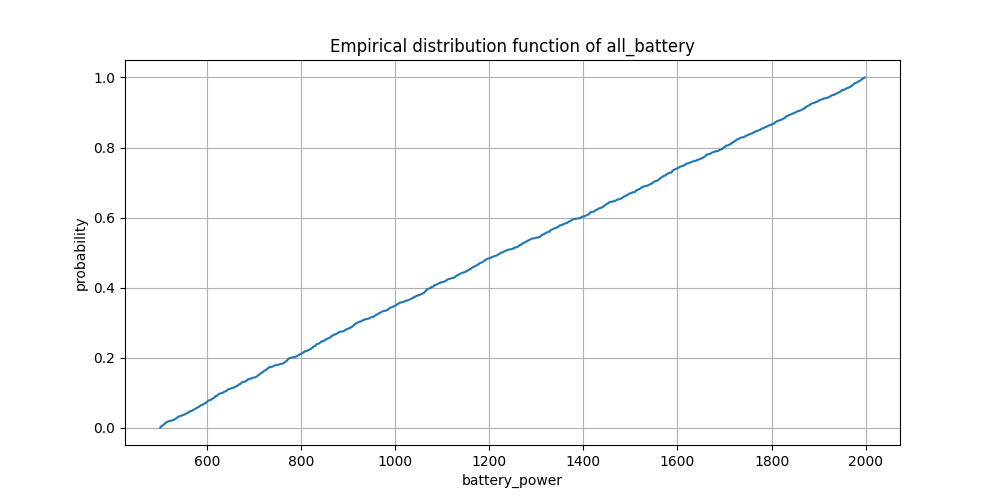
\includegraphics[scale=0.55]{all_battery_edf.png}
        \captionsetup{skip=0pt}
        \caption{График эмпирической функции распределения для всей выборки}
        \label{fig:allbedf}
    \end{figure}
    \begin{figure}[H]
        \centering
        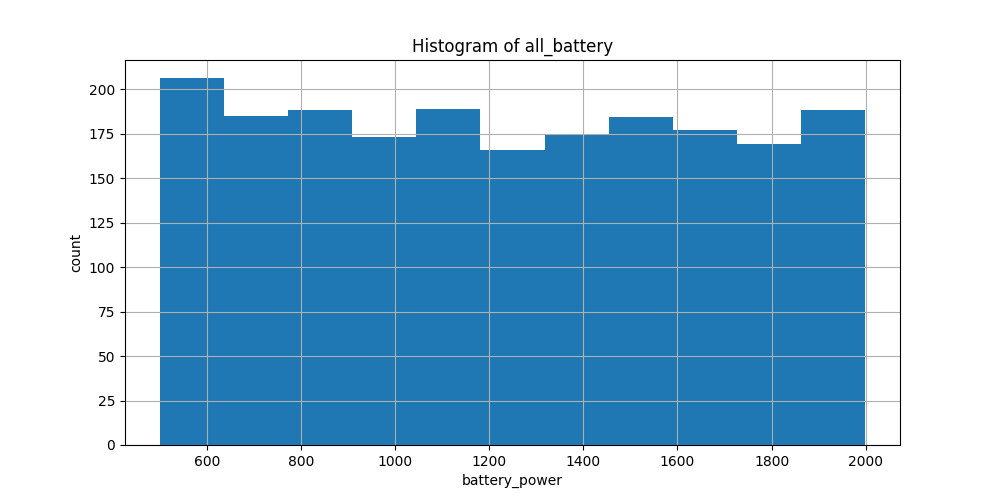
\includegraphics[scale=0.55]{all_battery_hist.png}
        \captionsetup{skip=0pt}
        \caption{Гистограмма для всей выборки}
        \label{fig:allbhist}
    \end{figure}
    \begin{figure}[H]
        \centering
        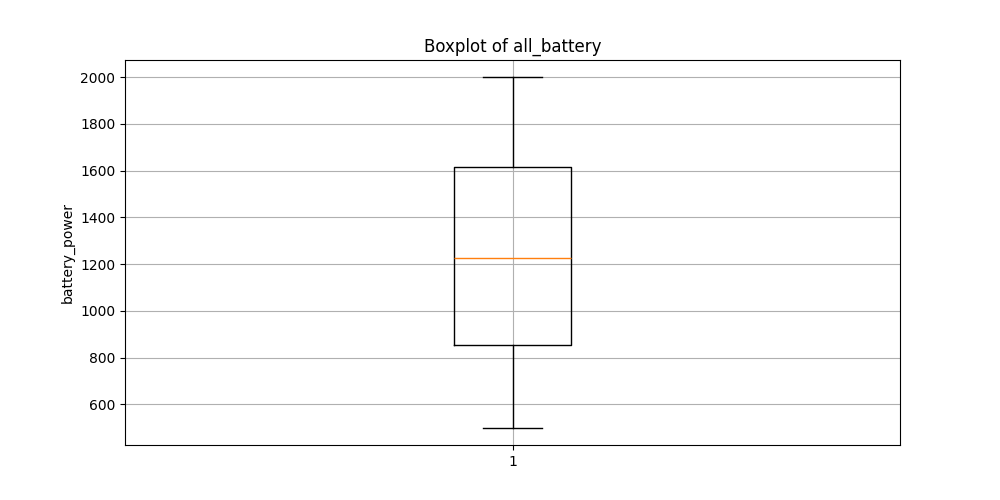
\includegraphics[scale=0.55]{all_battery_box.png}
        \captionsetup{skip=0pt}
        \caption{Ящик с усами для всей выборки}
        \label{fig:allbbox}
    \end{figure}


    \begin{figure}[H]
        \centering
        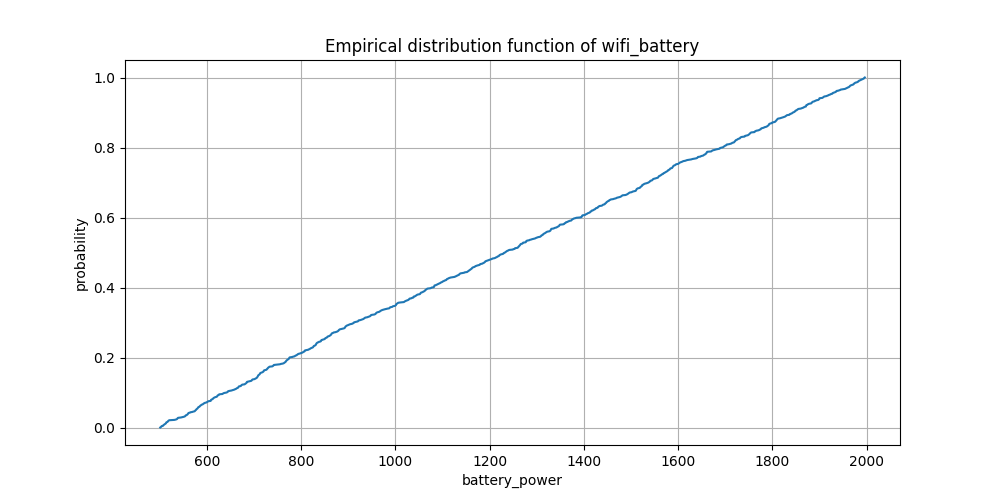
\includegraphics[scale=0.55]{wifi_battery_edf.png}
        \captionsetup{skip=0pt}
        \caption{График эмпирической функции распределения для выборки моделей с Wi-Fi}
        \label{fig:wifibedf}
    \end{figure}
    \begin{figure}[H]
        \centering
        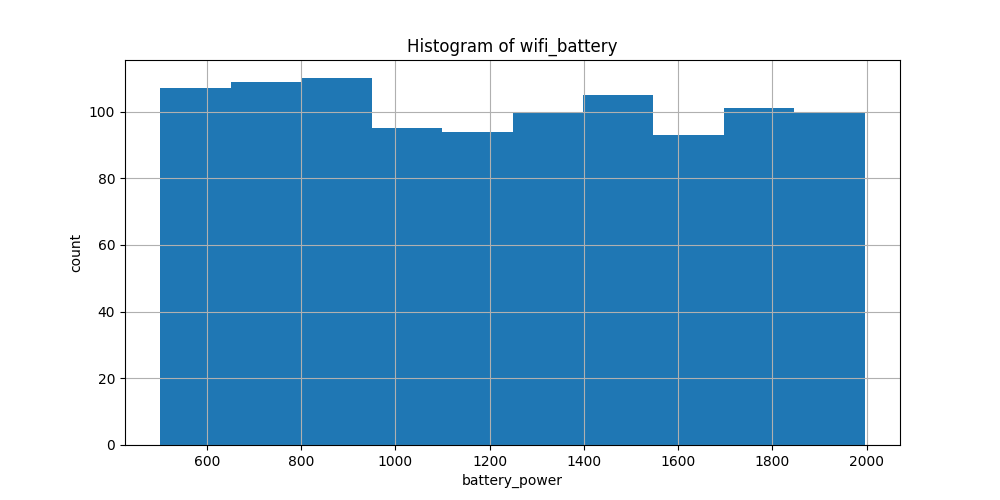
\includegraphics[scale=0.55]{wifi_battery_hist.png}
        \captionsetup{skip=0pt}
        \caption{Гистограмма для выборки моделей с Wi-Fi}
        \label{fig:wifibhist}
    \end{figure}
    \begin{figure}[H]
        \centering
        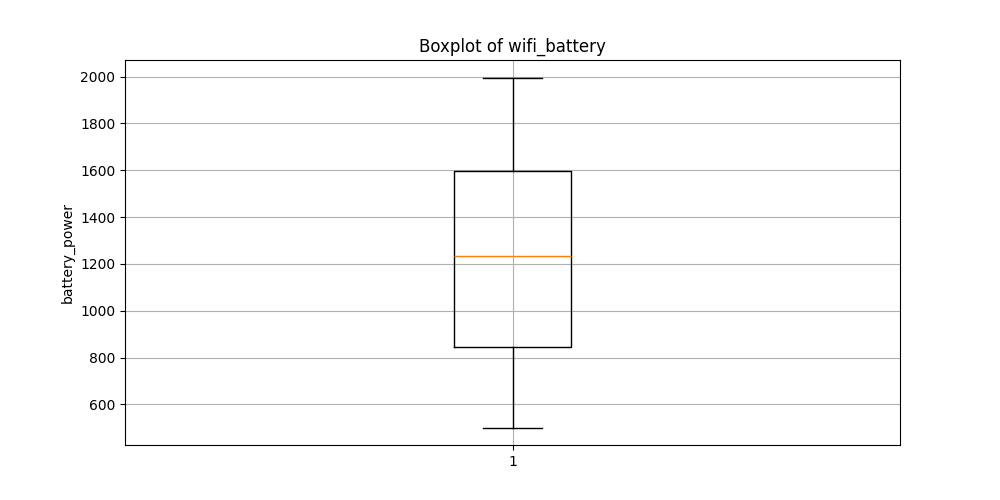
\includegraphics[scale=0.55]{wifi_battery_box.png}
        \captionsetup{skip=0pt}
        \caption{Ящик с усами для выборки моделей с Wi-Fi}
        \label{fig:wifibbox}
    \end{figure}


    \begin{figure}[H]
        \centering
        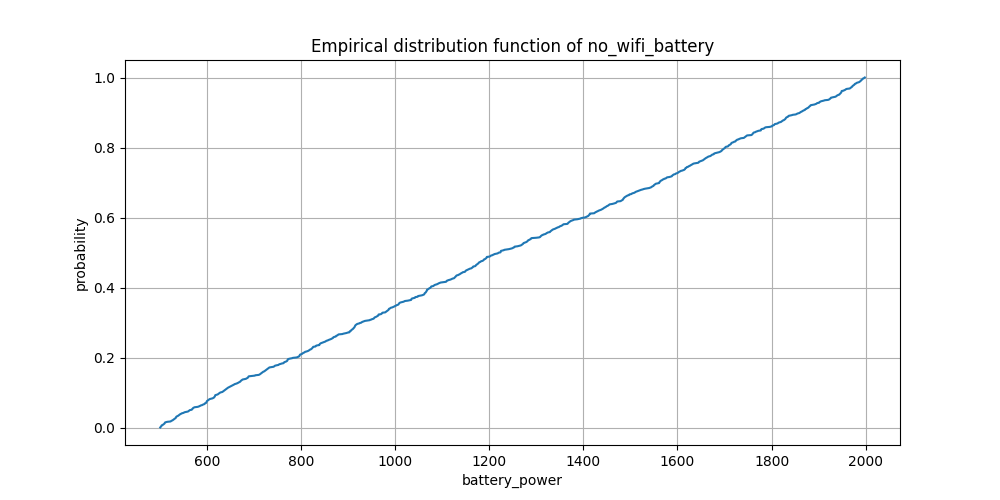
\includegraphics[scale=0.55]{no_wifi_battery_edf.png}
        \captionsetup{skip=0pt}
        \caption{График эмпирической функции распределения для выборки моделей без Wi-Fi}
        \label{fig:nowifibedf}
    \end{figure}
    \begin{figure}[H]
        \centering
        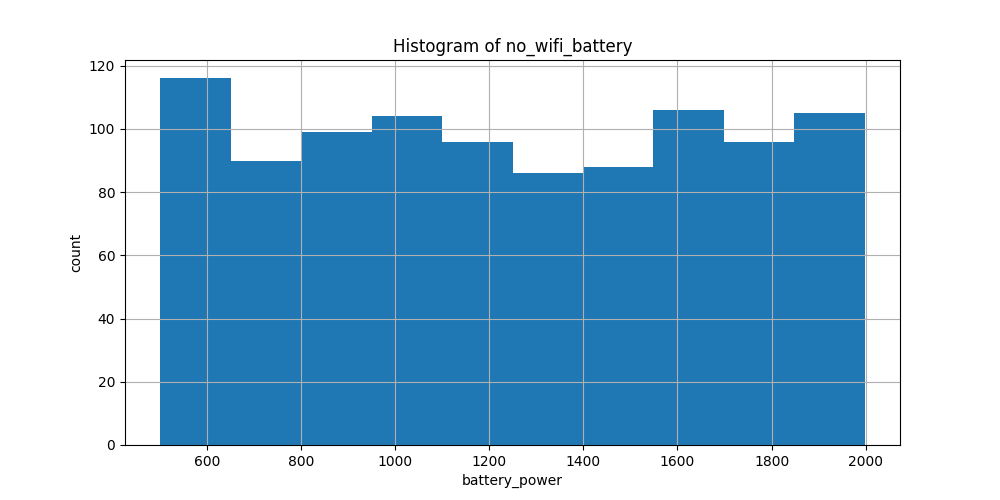
\includegraphics[scale=0.55]{no_wifi_battery_hist.png}
        \captionsetup{skip=0pt}
        \caption{Гистограмма для выборки моделей без Wi-Fi}
        \label{fig:nowifibhist}
    \end{figure}
    \begin{figure}[H]
        \centering
        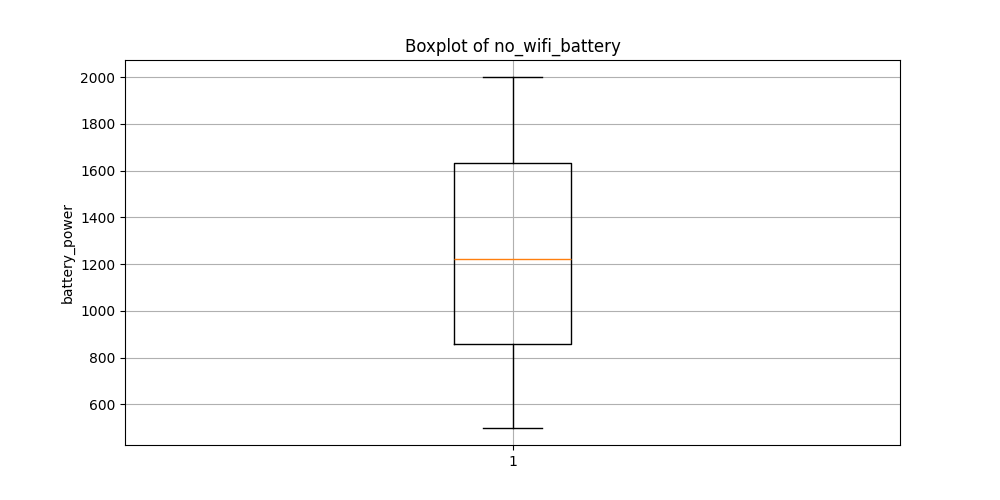
\includegraphics[scale=0.55]{no_wifi_battery_box.png}
        \captionsetup{skip=0pt}
        \caption{Ящик с усами для выборки моделей без Wi-Fi}
        \label{fig:nowifibbox}
    \end{figure}


    \newpage
    Исходя из результирующих графиков можно сделать вывод, что мы верно посчитали характеристики,
    представленные в листинге \ref{mvalsout}.
    На рис. \ref{fig:allbedf} вероятность всегда неубывает, медиана прослеживается
    в районе значения, посчитанного ранее. На рис. \ref{fig:allbhist} столбцы примерно одинаковой высоты --
    распределение скорее всего равномерное. На рис. \ref{fig:allbbox} медиана отмечена
    оранжвой прямой, находится примерно в центре ящика -- распределение данных относительно
    симметрично, и, ее значение совпадает с вычисленным. Интервал между минимумом и максимумом значений в ящике получился
    широким, что подтверждает большое значение вычисленной ранее дисперсии. Выбросы отсутствуют (нет точек вне усов).
    Рассуждения аналогичны для графиков с другой выборкой.


    \section{Задание 2}
    \subsection{Условие}
    Методом моментов найти оценку квадрата масштабирующего параметра $\theta$ распределения Лапласа
    (сдвиг считать нулевым). Эксперимент при $\theta=0.5$. \textbf{Указание}: для плотности используйте
    параметризацию $$f_{\theta}(x)=\dfrac{1}{2\theta}\exp{\left\{-\dfrac{|x|}{\theta}\right\}}$$


    Найти смещение, дисперсию, среднеквадратическую ошибку (\textbf{теоретические}) и указать свойства оценок.
    Также провести эксперимент при указанных параметрах по следующей схеме:
    \begin{enumerate}
        \item Задайте массив объемов выборки
        \item Для каждого объема выборки $n$ сгенерируйте $m$ выборок из вашего распределения и для каждой
        сгенерированной выборки посчитайте оценку параметра согласно полученной формуле
        \item Обработайте результаты (посчитайте выборочные характеристики для разницы между оценкой и реальным
        параметром для каждого объема выборки, количество выборок, для которых оценка отличается от реального
        параметра более чем на заданный вами порог и т. п.), визуализируйте результат
    \end{enumerate}


    \subsection{Выполнение}
    Чтобы найти $\hat{\theta}^2$ методом моментов, необходимо приравнять теоретический и эмпирический
    моменты порядка $k$. Теоретический выражается как функция от параметров распределения, которые мы
    оцениваем. Эмпирический определяется на основе данных выборки.


    Для начала определимся с тем, сколько нужно задать функций $g_i(x)$, по которым мы будем искать оценки $\hat{\theta_i}$
    параметров распределения -- нам известен сдвиг $\mu=0$ и нужно оценить только $\theta^2$, следовательно количество
    неизвестных $d=1$, а значит нам нужно задать одну функцию $g(x)$ и по ней найти одну оценку $\hat{\theta}^2$.


    Начнем с нахождения теоретического момента. Нам необходимо задать такую функцию $$g(x)=x^k,$$ которая
    при поиске $k$-го момента позволит нам получить выражение с $\theta^2$, чтобы после приравнивания моментов
    мы могли выразить оценку $\hat{\theta}^2$ этого параметра.


    Попробуем задать $g(x)=x$. В таком случае, согласно википедии, получим первый момент
    (математическое ожидание) для распределения Лапласа, равный(-ое)
    сдвигу $\mu$, который в нашем случае отсутствует
    $$\mathbb{E}\left[g(x)\right]=\mathbb{E}\left[x\right]=\mu=0$$
    С первым моментом выражения с $\theta^2$ не получилось. Тогда, пусть $g(x)=x^2$ -- теперь
    найдем второй момент для распределения Лапласа. Пользуясь википедией, получим
    $$\mathbb{E}\left[g(x)\right]=\mathbb{E}\left[x^2\right]=\int\limits_{-\infty}^{\infty}x^2f_{\theta}(x)\,dx=\mu^2+2\theta^2=/\mu=0/=2\theta^2$$
    Мы получили теоретический момент порядка $k=2$ для распределения Лапласа.
    
    
    Найдем эмпирический момент порядка $k=2$ для распределения Лапласа. Имеем на данный момент такое выражение
    $$\mathbb{E}\left[g(x)\right]=\mathbb{E}\left[x^2\right]=2\theta^2$$
    Запишем вместо математического ожидания $\mathbb{E}\left[x^2\right]$ выборочный аналог таким способом
    $$\mathbb{E}\left[g_i(x_j)\right]=\dfrac{1}{n}\sum\limits_{j=1}^{n}g_i(x_j)\Rightarrow \mathbb{E}\left[g(x_j)\right]=\mathbb{E}\left[x_j^2\right]=\dfrac{1}{n}\sum\limits_{j=1}^{n}x_j^2$$
    Полученное для $\mathbb{E}\left[x_j^2\right]$ выражение является эмпирическим вторым моментом для распределения Лапласа.


    Приравняем эмпирический и теоретический моменты второго порядка и выразим оценку квадрата параметра $\theta$
    $$\dfrac{1}{n}\sum\limits_{j=1}^{n}x_j^2=2\theta^2\Rightarrow\hat{\theta}^2=\dfrac{1}{2n}\sum\limits_{j=1}^{n}x_j^2$$


    Таким образом, методом моментов оценка квадрата масштабирующего параметра $\theta$ распределения Лапласа имеет вид
    $$\hat{\theta}^2=\dfrac{1}{2n}\sum\limits_{j=1}^{n}x_j^2$$
    Далее будем находить характеристики и проводить эксперименты с данным в условии значением $\theta=0.5$.


    Смещение можно найти по следующей формуле $$\text{bias}{\left[\hat{\theta},\,\theta\right]}=\mathbb{E}\left[\hat{\theta}\right]-\theta$$
    Если результат выражения выше равен нулю, значит оценка является несмещенной. В нашем случае имеем
    $$\text{bias}{\left[\hat{\theta}^2,\,\theta^2\right]}=\mathbb{E}\left[\hat{\theta}^2\right]-\theta^2$$
    Вычислим это выражение, применяя свойства математического ожидания. $\theta^2$ является
    константой и мы сразу можем ее вычислить. Рассмотрим подробнее $\mathbb{E}\left[\hat{\theta}^2\right]$
    $$\mathbb{E}\left[\hat{\theta}^2\right]=\mathbb{E}\left[\dfrac{1}{2n}\sum\limits_{j=1}^{n}x_j^2\right]=\dfrac{1}{2n}\mathbb{E}\left[\sum\limits_{j=1}^{n}x_j^2\right]
    =\dfrac{1}{2n}\sum\limits_{j=1}^{n}\mathbb{E}\left[x_j^2\right],$$
    $$\sum\limits_{j=1}^{n}\mathbb{E}\left[x_j^2\right]=
    \begin{bmatrix}
        \mathbb{E}\left[x^2\right]=2\theta^2\\
        \mathbb{E}\left[x_1^2\right]=2\theta^2\\
        \vdots \\
        \mathbb{E}\left[x_n^2\right]=2\theta^2
    \end{bmatrix}=
    n\cdot2\theta^2,
    $$
    $$\dfrac{1}{2n}\sum\limits_{j=1}^{n}\mathbb{E}\left[x_j^2\right]=\dfrac{1}{2n}\cdot n\cdot2\theta^2=\theta^2
    \Rightarrow \mathbb{E}\left[\hat{\theta}^2\right]=\theta^2$$
    Теперь вычислим смещение
    $$\text{bias}{\left[\hat{\theta}^2,\,\theta^2\right]}=\mathbb{E}\left[\hat{\theta}^2\right]-\theta^2=\theta^2-\theta^2=0$$
    Таким образом, оценка является несмещенной.


    Вычислим теоретическую дисперсию оценки, пользуясь свойствами дисперсии и математического ожидания. В ходе вычислений вспомним биномиальный коэффициент и гамма функцию
    $$\text{Var}{\left[\hat{\theta}^2\right]}=\mathbb{E}\left[\hat{\theta}^4\right]-\left(\mathbb{E}\left[\hat{\theta}^2\right]\right)^2
    =\begin{bmatrix}
        \mathbb{E}\left[\hat{\theta}^2\right]=\theta^2\\
        \mathbb{E}\left[\hat{\theta}^4\right]=\mathbb{E}\left[\left(\hat{\theta}^2\right)^2\right]
    \end{bmatrix}
    =\mathbb{E}\left[\left(\dfrac{1}{2n}\sum\limits_{j=1}^{n}x_j^2\right)^2\right]-\left(\theta^2\right)^2,$$
    $$\mathbb{E}\left[\left(\dfrac{1}{2n}\sum\limits_{j=1}^{n}x_j^2\right)^2\right]=\dfrac{1}{4n^2}\mathbb{E}\left[\left(\sum\limits_{j=1}^{n}x_j^2\right)^2\right],$$
    $$\left(\sum\limits_{j=1}^{n}x_j^2\right)^2=\sum\limits_{j=1}^{n}x_j^4+2\sum\limits_{i\neq j}x_i^2x_j^2\Rightarrow \mathbb{E}\left[\hat{\theta}^4\right]=\dfrac{1}{4n^2}\mathbb{E}\left[\sum\limits_{j=1}^{n}x_j^4+2\sum\limits_{i\neq j}x_i^2x_j^2\right],$$
    $$\mathbb{E}\left[\sum\limits_{j=1}^{n}x_j^4+2\sum\limits_{i\neq j}x_i^2x_j^2\right]=\mathbb{E}\left[\sum\limits_{j=1}^{n}x_j^4\right]+\mathbb{E}\left[2\sum\limits_{i\neq{j}}x_i^2x_j^2\right]=
    \sum\limits_{j=1}^{n}E\left[x_j^4\right]+2\sum\limits_{i\neq{j}}\mathbb{E}\left[x_i^2x_j^2\right],$$
    $$\sum\limits_{i\neq{j}}\mathbb{E}\left[x_i^2x_j^2\right]=/\text{случ. вел. }x_i \text{ независимы}/=\sum\limits_{i\neq{j}}\mathbb{E}\left[x_i^2\right]\mathbb{E}\left[x_j^2\right],$$
    $$2\sum\limits_{i\neq{j}}\mathbb{E}\left[x_i^2x_j^2\right]=2\sum\limits_{i\neq{j}}\mathbb{E}\left[x_i^2\right]\mathbb{E}\left[x_j^2\right]=/\mathbb{E}\left[x^2\right]=2\theta^2/=2\sum\limits_{i\neq{j}}2\theta^2\cdot2\theta^2=8\theta^4\sum\limits_{i\neq{j}}1,$$
    $$\sum\limits_{i\neq{j}}1=
    /\text{бином. коэфф.}/=
    \begin{pmatrix}
        n\\
        k=2>0
    \end{pmatrix}
    =\dfrac{n\left(n-1\right)}{2},$$
    $$2\sum\limits_{i\neq{j}}\mathbb{E}\left[x_i^2x_j^2\right]=8\theta^4\cdot\dfrac{n\left(n-1\right)}{2}=4\theta^4n\left(n-1\right),$$
    $$\sum\limits_{j=1}^{n}\mathbb{E}\left[x_j^4\right]=
    \begin{bmatrix}
        \mathbb{E}\left[x^4\right]=\alpha\\
        \mathbb{E}\left[x_1^4\right]=\alpha\\
        \vdots \\
        \mathbb{E}\left[x_n^4\right]=\alpha
    \end{bmatrix}=
    n\cdot\mathbb{E}\left[x^4\right],\text{ где }\mathbb{E}\left[x^4\right]\text{ -- четвертый момент},$$
    $$\mathbb{E}\left[x^4\right]=\int\limits_{-\infty}^{\infty}x^4f_{\theta}(x)\,dx=\int\limits_{-\infty}^{\infty}x^4\cdot\dfrac{1}{2\theta}\exp{\left\{-\dfrac{|x|}{\theta}\right\}}\,dx=\dfrac{1}{2\theta}\int\limits_{-\infty}^{\infty}x^4\exp{\left\{-\dfrac{|x|}{\theta}\right\}}\,dx$$
    Так как в нашем распределении Лапласа сдвиг отсутствует ($\mu=0$), то это означает, что распределение симметрично относительно нуля. Тогда, вычислим интеграл только для
    положительных значений $x$ и умножим его на два. При условии $x\geq0$ получаем $|x|=x$
    $$\mathbb{E}\left[x^4\right]=\dfrac{1}{2\theta}\int\limits_{-\infty}^{\infty}x^4\exp{\left\{-\dfrac{|x|}{\theta}\right\}}\,dx=2\cdot\dfrac{1}{2\theta}\int\limits_{0}^{\infty}x^4\exp{\left\{-\dfrac{x}{\theta}\right\}}\,dx=
    \dfrac{1}{\theta}\int\limits_{0}^{\infty}x^4\exp{\left\{-\dfrac{x}{\theta}\right\}}\,dx,$$
    $$\dfrac{1}{\theta}\int\limits_{0}^{\infty}x^4\exp{\left\{-\dfrac{x}{\theta}\right\}}\,dx=
    \begin{bmatrix}
        u=\dfrac{x}{\theta}\\
        du=\dfrac{dx}{\theta}
    \end{bmatrix}=
    \dfrac{1}{\theta}\int\limits_{0}^{\infty}u^4\theta^4e^{-u}\theta\,du=\theta^4\int\limits_{0}^{\infty}u^4e^{-u}\,du=\theta^4\cdot\Gamma{(z)},$$
    $$\Gamma{(z)}=\int\limits_{0}^{\infty}t^{z-1}e^{-t}\,dt\Rightarrow\int\limits_{0}^{\infty}u^4e^{-u}\,du=\Gamma{(z-1=4)}=\Gamma{(5)}=24\Rightarrow\mathbb{E}\left[x^4\right]=\theta^4\cdot\Gamma{(5)}=\theta^4\cdot24,$$
    $$\sum\limits_{j=1}^{n}\mathbb{E}\left[x_j^4\right]=n\cdot\mathbb{E}\left[x^4\right]=n\cdot\theta^4\cdot24,$$
    $$\mathbb{E}\left[\hat{\theta}^4\right]=\dfrac{1}{4n^2}\left(\sum\limits_{j=1}^{n}E\left[x_j^4\right]+2\sum\limits_{i\neq{j}}\mathbb{E}\left[x_i^2x_j^2\right]\right)=
    \dfrac{1}{4n^2}\left(24\theta^4n+4\theta^4n\left(n-1\right)\right),$$
    $$\dfrac{1}{4n^2}\left(24\theta^4n+4\theta^4n\left(n-1\right)\right)=\dfrac{4\theta^4n}{4n^2}\left(6+n-1\right)=\dfrac{\theta^4}{n}\left(n+5\right)=\theta^4\left(1+\dfrac{5}{n}\right)=\mathbb{E}\left[\hat{\theta}^4\right],$$
    $$\text{Var}{\left[\hat{\theta}^2\right]}=\mathbb{E}\left[\hat{\theta}^4\right]-\left(\mathbb{E}\left[\hat{\theta}^2\right]\right)^2=
    \theta^4\left(1+\dfrac{5}{n}\right)-\theta^4=\theta^4\left(1+\dfrac{5}{n}-1\right)=\dfrac{5\theta^4}{n}$$
    При условии, что эксперимент проводится для $\theta=0.5$, получим
    $$\text{Var}{\left[\hat{\theta}^2\right]}=\dfrac{5\cdot0.5^4}{n}=\dfrac{0.3125}{n}$$
    На самом деле, вследствие независимости случайных величин $x_i$ достаточно было вычислить выражение ниже, чтобы избежать лишних шагов, так как ковариации между независимыми случайными величинами равны нулю
    $$\text{Var}{\left[\hat{\theta}^2\right]}=\text{Var}{\left[\dfrac{1}{2n}\sum\limits_{j=1}^{n}x_j^2\right]}=\dfrac{1}{4n^2}\left(\sum\limits_{j=1}^{n}\text{Var}\left[x_{j}^2\right]+2\sum\limits_{i\neq{j}}\text{Cov}\,\left[x_i^2,x_j^2\right]\right)=\dfrac{1}{4n^2}\sum\limits_{j=1}^{n}\text{Var}\left[x_{j}^2\right]$$

    
    Найдем теоретическую среднеквадратическую ошибку. Так как оценка является несмещенной, то теоретические среднеквадратическая ошибка и дисперсия равны. Таким образом, получим
    $$\text{MSE}{\left[\hat{\theta}^2\right]}=\text{Var}{\left[\hat{\theta}^2\right]}=\dfrac{0.3125}{n}$$


    Далее распишем свойства оценки. Мы уже знаем, что оценка является \textbf{несмещенной}, так как смещение $\text{bias}{\left[\hat{\theta}^2,\,\theta^2\right]}=0$ ($\mathbb{E}\left[\hat{\theta^2}\right]=\theta^2$), т. е. отсутствует.


    Проверим состоятельность оценки
    $$\lim\limits_{n\rightarrow\infty}\text{MSE}{\left[\hat{\theta}^2\right]}=\lim\limits_{n\rightarrow\infty}\text{Var}{\left[\hat{\theta}^2\right]}=\lim\limits_{n\rightarrow\infty}\dfrac{0.3125}{n}=\left\{\dfrac{0.3125}{\infty}\right\}=0,$$
    из чего следует, что оценка является \textbf{состоятельной}, так как чем больше данных, тем более точной становится оценка.


    Проверим эффективность оценки с помощью нижней оценки дисперсии. Для этого понадобится неравенство Крамера-Рао
    $$\text{Var}{\left[\hat{\theta}^2\right]}\geq\dfrac{1}{I_n(\theta)}=\dfrac{1}{n\cdot I(\theta)},$$
    где $I(\theta)$ -- информация Фишера
    $$I(\theta)=\mathbb{E}\left[\dfrac{\partial\ln{L\left(\theta,x\right)}}{\partial\theta}\right]^2=-\mathbb{E}\left[\dfrac{\partial^2\ln{L\left(\theta,x\right)}}{\partial\theta^2}\right],$$
    где $L\left(\theta,x\right)=L\left(\theta,\,x_1,\,x_2,\,\hdots,\,x_n\right)$ -- функция правдоподобия. В нашем случае $L$ будет иметь вид
    $$L\left(\theta,x\right)=\prod_{i=1}^nf_{\theta}\left(x_i\right)=\left(\dfrac{1}{2\theta}\right)^n\exp{\left\{-\dfrac{1}{\theta}\sum{|x_i|}\right\}},$$
    теперь найдем логарифм функции правдоподобия. Это нужно для упрощения дифференцирования
    $$\ln{L\left(\theta,x\right)}=\ln{\dfrac{1}{\left(2\theta\right)^n}}\exp{\left\{-\dfrac{1}{\theta}\sum{|x_i|}\right\}}=\ln{\exp{\left\{-\dfrac{1}{\theta}\sum{|x_i|}\right\}}}-\ln{\left(2\theta\right)^n},$$
    $$\ln{\exp{\left\{-\dfrac{1}{\theta}\sum{|x_i|}\right\}}}=-\dfrac{1}{\theta}\sum{|x_i|},\ \ \ln{\left(2\theta\right)^n}=n\ln{2\theta},$$
    $$\ln{L\left(\theta,x\right)}=-\dfrac{1}{\theta}\sum{|x_i|}-n\ln{2\theta}$$
    Теперь последовательно два раза возьмем производную от $\ln{L\left(\theta,x\right)}$ по $\theta$
    $$\dfrac{\partial\ln{L\left(\theta,x\right)}}{\partial\theta}=\left(-\dfrac{1}{\theta}\sum{|x_i|}-n\ln{2\theta}\right)^{\prime}_{\theta}=
    \left(-\dfrac{1}{\theta}\sum{|x_i|}\right)^{\prime}_{\theta}-\left(n\ln{2\theta}\right)^{\prime}_{\theta},$$
    $$\left(-\dfrac{1}{\theta}\sum{|x_i|}\right)^{\prime}_{\theta}=\dfrac{1}{\theta^2}\sum{|x_i|}, \ \ \left(n\ln{2\theta}\right)^{\prime}_{\theta}=n\cdot\dfrac{2}{2\theta}=\dfrac{n}{\theta},$$
    $$\dfrac{\partial\ln{L\left(\theta,x\right)}}{\partial\theta}=\dfrac{1}{\theta^2}\sum{|x_i|}-\dfrac{n}{\theta},$$
    $$\dfrac{\partial^2\ln{L\left(\theta,x\right)}}{\partial\theta^2}=\left(\dfrac{1}{\theta^2}\sum{|x_i|}-\dfrac{n}{\theta}\right)^{\prime}_{\theta}=
    \left(\dfrac{1}{\theta^2}\sum{|x_i|}\right)^{\prime}_{\theta}-\left(\dfrac{n}{\theta}\right)^{\prime}_{\theta},$$
    $$\left(\dfrac{1}{\theta^2}\sum{|x_i|}\right)^{\prime}_{\theta}=-\dfrac{2}{\theta^3}\sum{|x_i|}, \ \ \left(\dfrac{n}{\theta}\right)^{\prime}_{\theta}=-\dfrac{n}{\theta^2}$$
    $$\dfrac{\partial^2\ln{L\left(\theta,x\right)}}{\partial\theta^2}=-\dfrac{2}{\theta^3}\sum{|x_i|}+\dfrac{n}{\theta^2}$$
    Теперь вычислим информацию Фишера $I\left(\theta\right)$
    $$I\left(\theta\right)=-\mathbb{E}\left[-\dfrac{2}{\theta^3}\sum{|x_i|}+\dfrac{n}{\theta^2}\right]=\mathbb{E}\left[\dfrac{2}{\theta^3}\sum{|x_i|}\right]-\mathbb{E}\left[\dfrac{n}{\theta^2}\right],$$
    $$\mathbb{E}\left[\dfrac{2}{\theta^3}\sum{|x_i|}\right]=\dfrac{2}{\theta^3}\mathbb{E}\left[\sum{|x_i|}\right]=\dfrac{2}{\theta^3}\sum{\mathbb{E}\left[|x_i|\right]}=\dfrac{2}{\theta^3}\cdot n\cdot\mathbb{E}\left[|x|\right],$$
    $$\mathbb{E}\left[|x|\right]=\int\limits_{-\infty}^{\infty}|x|f_{\theta}(x)\,dx=/\mu=0,\text{ распр. симм. относ. 0},\,|x|=x/=2\int\limits_{0}^{\infty}xf_{\theta}(x)\,dx,$$
    $$2\int\limits_{0}^{\infty}xf_{\theta}(x)\,dx=2\int\limits_{0}^{\infty}x\dfrac{1}{2\theta}\exp{\left\{\dfrac{-|x|}{\theta}\right\}}\,dx=\dfrac{1}{\theta}\int\limits_{0}^{\infty}x\exp{\left\{-\dfrac{x}{\theta}\right\}}\,dx,$$
    $$\dfrac{1}{\theta}\int\limits_{0}^{\infty}x\exp{\left\{-\dfrac{x}{\theta}\right\}}\,dx=\begin{bmatrix}
        u=\dfrac{x}{\theta}\\
        du=\dfrac{dx}{\theta}
    \end{bmatrix}=
    \dfrac{1}{\theta}\int\limits_{0}^{\infty}u\theta e^{-u}\theta\,du=\theta\int\limits_{0}^{\infty}ue^{-u}\,du=\theta\cdot\Gamma(z),$$
    $$\int\limits_{0}^{\infty}ue^{-u}\,du=\Gamma(z-1=1)=\Gamma(z=2)=1\Rightarrow\theta\cdot\Gamma(2)=\theta\Rightarrow\mathbb{E}\left[|x|\right]=\theta,$$
    $$\mathbb{E}\left[\dfrac{2}{\theta^3}\sum{|x_i|}\right]=\dfrac{2}{\theta^3}\cdot n\cdot\theta=\dfrac{2n}{\theta^2},\ \ \mathbb{E}\left[\dfrac{n}{\theta^2}\right]=\dfrac{n}{\theta^2},$$
    $$I\left(\theta\right)=\dfrac{2n}{\theta^2}-\dfrac{n}{\theta^2}=\dfrac{n}{\theta^2}\Rightarrow I_n\left(\theta\right)=n\cdot\dfrac{n}{\theta^2}=\dfrac{n^2}{\theta^2}\Rightarrow\dfrac{1}{I_n(\theta)}=\dfrac{\theta^2}{n^2}$$
    Таким образом, получим
    $$\text{Var}{\left[\hat{\theta}^2\right]}\geq \dfrac{\theta^2}{n^2}\Rightarrow\dfrac{5\theta^4}{n}\geq \dfrac{\theta^2}{n^2}\Rightarrow 5\theta^2\geq \dfrac{1}{n},$$
    из чего следует, что $\forall n:5\theta^2>\frc{1}{n}$, что означает, что оценка является \textbf{неэффективной}.


    Проверим асимптотическую нормальность. Так как случайные величины
    независимы, одинаково распределены (все случ. вел. $x_i$ имеют одно и то же распределение с одинаковыми мат. ожиданиями и дисперсией),
    имеют конечные математическое ожидание и дисперсию,
    и, дисперсия среднего (то есть дисперсия квадрата оценки масштабирующего параметра $\theta$) с увеличенем объема выборки уменьшается,
    то, по центральной предельной теореме (ЦПТ) сумма (или среднее) этих случайных величин при $n\rightarrow\infty$ будет приближаться по распределению $d$ к нормальному распределению,
    то есть $$\sqrt{n}\left(\hat{\theta}-\theta\right)\xrightarrow{d}\mathcal{N}\left(0,\sigma^2\left[\theta\right]\right),$$ что в нашем случае будет иметь вид
    $$\sqrt{n}\left(\hat{\theta}^2-\theta^2\right)\xrightarrow{d}\mathcal{N}\left(0,\text{Var}{\left[\hat{\theta}^2\right]}\right),$$
    $$\sqrt{n}\left(\dfrac{1}{2n}\sum\limits_{j=1}^{n}x_{j}^2-\theta^2\right)\xrightarrow{d}\mathcal{N}\left(0,\dfrac{5\theta^4}{n}\right),$$
    где $\dfrac{1}{2n}\sum\limits_{j=1}^{n}x_{j}^2$ -- среднее квадратичных отклонений. Следовательно, оценка является \textbf{асимптотически нормальной}.


    Проведем эксперимент при указанных параметрах на языке программирования \texttt{Python}. Импортируем необходимые для эксперимента библиотеки (и оставляем метод для разделения вывода)
    \begin{lstlisting}[label=import2, caption={Импортирование библиотек для эксперимента}]
    import numpy as np
    import matplotlib.pyplot as plt

    # common separator between unrelated outputs
    def print_separate():
        print('----------------')
    \end{lstlisting}


    Зададим основные переменные: \texttt{n\_{list}} содержит различные объемы выборки, \texttt{m} -- кол-во выборок распределения Лапласа,
    \texttt{theta} -- истинное значение масштабирующего параметра, \texttt{delta} -- порог для определения смещения, \texttt{hat\_theta2\_dict}
    -- словарь, в котором для каждого $n_i$ (ключа -- объема выборки) определен свой пустой список (значение -- оценка квадрата параметра). 
    \begin{lstlisting}[label=main_variables, caption={Определение основных переменных в программе}]
    n_list = [10, 100, 1000]  # list of sample sizes
    m = 100  # number of samples for each n
    theta = 0.5  # true value of the scaling parameter
    delta = 0.1  # threshold for determining the difference
    hat_theta2_dict = {n: [] for n in n_list} # dictionary (key-val) for
                                              # storing estimates
    \end{lstlisting}


    Сгенерируем выборки в соответствии с заданием и посчитаем оценки
    \begin{lstlisting}[label=gen_calc, caption={Код для генерации выборок и подсчета оценок выведенной формулой}]
    # for each n generating m samples 
    # and calculating estimates
    for n in n_list:
        for i in range(m):
            # generating a sample (Laplace, bias=0)
            sample = np.random.laplace(loc=0, scale=theta, size=n)
                
            # calc hat_theta^2 accroding to the derived formula
            hat_theta2 = (1 / (2 * n)) * np.sum(sample ** 2)
            hat_theta2_dict[n].append(hat_theta2)
    \end{lstlisting}


    Обработаем результаты в соответствии с заданием. Посчитаем матожидание и дисперсию для разницы
    между оценкой и реальным параметром. Подсчитаем оценки, не попавшие в диапазон $\left(-\delta,\delta\right)$.
    Запишем результаты в новый словарь, чтобы после удобно вывести их в консоль, а также построить графики
    \begin{lstlisting}[label=proc_res, caption={Подсчет выборочных характеристик смещения и количество отличиий оценки от реального параметра на порог}]
    # processing results
    results = {}
    for n in n_list:
        hat_theta2_arr = np.array(hat_theta2_dict[n])
            
        # difference between estimate and true value
        bias = hat_theta2_arr - theta**2
            
        # sample characteristics
        mean_bias = np.mean(bias)
        var_bias = np.var(bias)
        biased_count = np.sum(np.abs(bias) > delta) # Number of samples that
                                                    # exceed the threshold
            
        results[n] = {
            'mean_bias': mean_bias,
            'var_bias': var_bias,
            'biased_count': biased_count,
            'hat_theta2_arr': hat_theta2_arr
        }
    \end{lstlisting}


    Выведем результаты в коноль следующим кодом
    \begin{lstlisting}[label=res2, caption={Код для вывода в консоль результатов эксперимента}]
    # results output
    print(f"m={m}")
    for n in n_list:
        print_separate()
        print(f"n={n}")
        print(f"mean_bias: {results[n]['mean_bias']:.4f}")
        print(f"var_bias: {results[n]['var_bias']:.4f}")
        print(f"biased_count: {results[n]['biased_count']}")
    \end{lstlisting}


    Получим такие результаты. Видим, что при увеличении объема выборки дисперсия и количество отклоненных оценок уменьшаются
    \begin{lstlisting}[label=res2out, caption={Вывод результатов эксперимента в консоль}]
    m=100
    ----------------  
    n=10
    mean_bias: -0.0073
    var_bias: 0.0224  
    biased_count: 50  
    ----------------  
    n=100
    mean_bias: -0.0031
    var_bias: 0.0024
    biased_count: 5
    ----------------
    n=1000
    mean_bias: -0.0003
    var_bias: 0.0004
    biased_count: 0
    \end{lstlisting}


    Вместе с этим для тех же данных выполнится код для построения гистограмм и ящиков с усами -- визуализируем результаты.
    Шаги построения графиков аналогичны первому заданию
    \begin{lstlisting}[label=graphs2, caption={Код для визуализации результатов}]
    # visualisation
    plt.figure(figsize=(10, 5))

    # building hist
    for n in n_list:
        plt.hist(results[n]['hat_theta2_arr'], 
                bins=np.int64(np.floor(1 + 3.322 * np.log10(n))), # Sturges'
                                                                  # rule
                alpha=0.5, 
                label=f'n={n}')

    plt.axvline(x=theta**2, color='red', linestyle='--',
                label=r'true value of $\theta^2$')
    plt.title(r'Distribution of $\theta^2$ estimates for different\
              sample sizes')
    plt.xlabel(r'$\hat{\theta}^2$')
    plt.ylabel('count')
    plt.legend()
    plt.grid()
    plt.show()

    # building boxplot
    plt.figure(figsize=(10, 5))
    plt.boxplot([results[n]['hat_theta2_arr'] for n in n_list],
                labels=n_list)
    plt.title(r'Boxplot of $\theta^2$ estimates for different n')
    plt.ylabel(r'$\hat{\theta}^2$')
    plt.xlabel('sample size n')
    plt.grid()
    plt.show()
    \end{lstlisting}


    \begin{figure}[H]
        \centering
        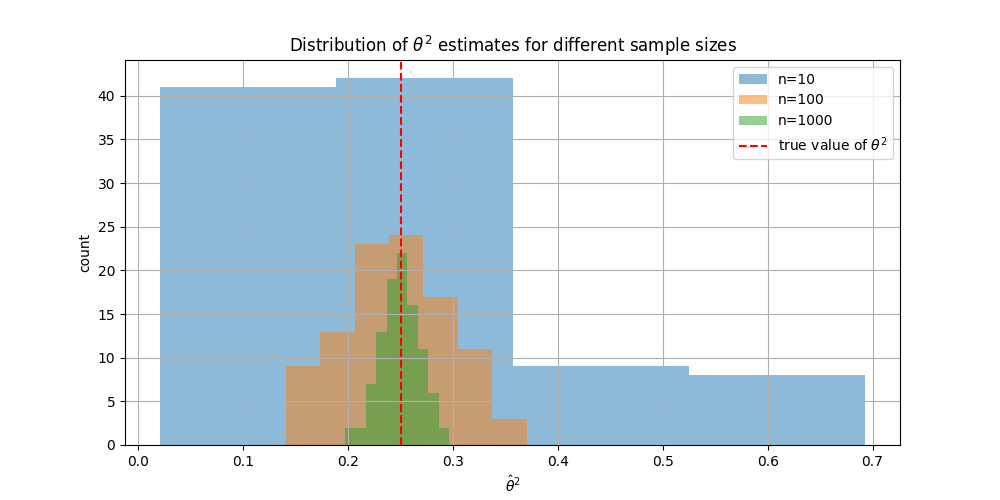
\includegraphics[scale=0.55]{hist_10_100_1000.png}
        \captionsetup{skip=0pt}
        \caption{Гистограммы для различных объемов выборки}
        \label{fig:hist}
    \end{figure}
    \begin{figure}[H]
        \centering
        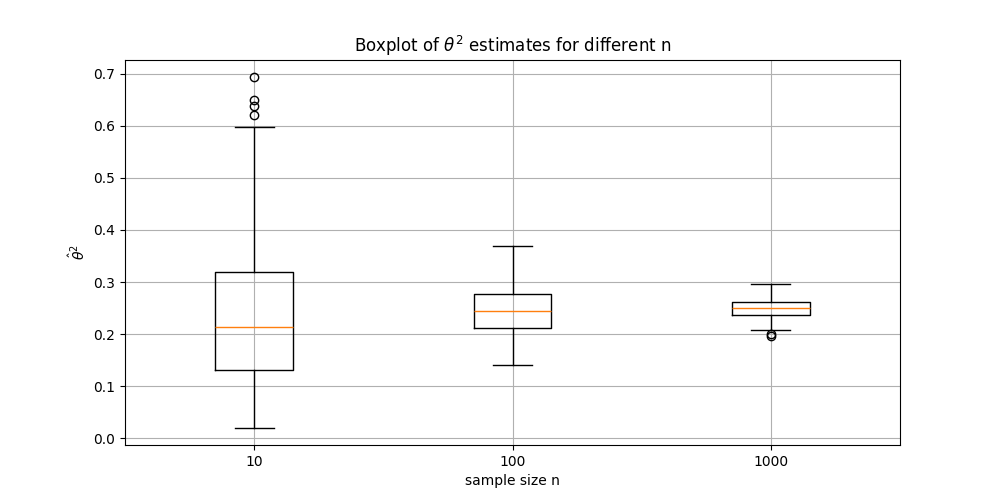
\includegraphics[scale=0.55]{boxplot_10_100_1000.png}
        \captionsetup{skip=0pt}
        \caption{Ящики с усами для различных объемов выборки}
        \label{fig:boxplot}
    \end{figure}
    

    Как видим, распределение стремится к нормальному с увеличенем объема выборки, разброс становится меньше, однако это не исключает
    возможности появления выбросов, медиана почти не меняет своего значения при увеличении $n$ со 100 до 1000, сжатие ящиков говорит
    о сходимости оценок к истинному значению параметра. В целом наши вычисления, рассуждения и выводы, проделанные в этом задании,
    подтвердились.
\end{document}